% !TEX encoding = UTF-8 Unicode
% !TEX root = ../rapport.tex

\chapter{Analyse et reflexion}\label{Analyse_et_reflexion}


\section{Critique de l'existant}


\section{Modèle choisi}

\begin{figure}[h]
\centering
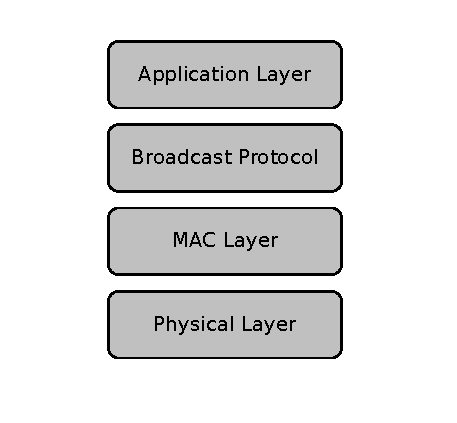
\includegraphics[scale=0.9]{Etat_de_l'art/source/layer.pdf}
\caption{\label{Layer} Les couches dans les WSNs}
\end{figure}

Pour l'étude et la conception d'algorithmes dans les réseaux de capteurs sans fil (WSN), il est indispensable de définir le problème précis, d'établir un cadre rigoureux, formel et sans ambiguïtés. Au vue de la figure \ref{Layer}, notre étude se placera dans la couche 'Broadcast Protocols'. Nous ne développerons pas la couche MAC ni la couche application.

Dans le cadre de notre travail d'étude et de recherche, nous utiliserons, sauf mention du contraire, la modélisation de capteurs simplifiée $M_1$ (cf \ref{modelePratique}) avec pour modèle énergétique celui décrit précédemment.
% TODO : on a choisi le broadcast, …
 


\section{Nos idées}

\subsection{Application du rayon optimal à DLBIP}
\begin{algorithm}[h]
\caption{DLBIP avec rayon optimal}
\label{algo_DLBIP}
\begin{algorithmic}
\STATE ENTREES  $G=(V,E)$ un graphe connexe, $s$ une source, un message $M$
\STATE SORTIE  DLBIP Broadcast
\STATE REQUIE  Connaissance du 2-voisinage
\STATE $R_{opt}=\sqrt[\alpha]{\frac{2c}{\alpha-2}}$
\STATE $s$ calcul son BIP($N_2(s),s,P'_{ij}$) et diffuse <M,$s$> à ses fils
\IF{ $u$ recoit <M,$v$> :}
	\IF{Le paquet contient des instruction pour $u$}
		\STATE $u$ construit BIP($N_2(u),u,P'_{ij}$) est retransmet le message à ses fils avec pour rayon:
			  \STATE - $R_{opt}$ si $\max\limits_{v\in N_u(1)\bigcap BIP(N_2(u),u,P'_{ij}}(d_e(u,v)< R_{opt}$
			  \STATE - $\max\limits_{v\in N_u(1)\bigcap BIP(N_2(u),u,P'_{ij}}(d_e(u,v)$ sinon.
			  
	\ENDIF
\ENDIF
\end{algorithmic}
\end{algorithm}










